\documentclass[aspectratio=169,11pt]{beamer}

\usepackage[T1]{fontenc}
\usepackage[utf8]{inputenc}
\usepackage[english]{babel}
\usepackage{newtxtext}
\usepackage{newtxmath}
\usepackage{graphicx}
\usepackage{booktabs}
\usepackage{xcolor}
\usepackage[numbers]{natbib}

\definecolor{accent}{RGB}{23,68,110}

\usetheme{Madrid}
\usecolortheme{seahorse}
\usefonttheme{professionalfonts}
\setbeamertemplate{navigation symbols}{}
\setbeamertemplate{items}[circle]
\setbeamertemplate{bibliography item}[text]
\setbeamercolor{structure}{fg=accent}

\title[Retrieval-Augmented Reward Modeling]{Retrieval-Augmented Reward Modeling}
\subtitle[Proposal + Weekly Update]{Long-Horizon Robot Manipulation in Simulation\\Proposal Overview + Weekly Execution Update}
\author[RAG-cross-RL]{RAG-cross-RL}
\date[Apr 1, 2026]{April 1, 2026}

\begin{document}

\begin{frame}[plain]
  \titlepage
\end{frame}

\begin{frame}{Outline}
  \tableofcontents
\end{frame}

\section{Background}
\begin{frame}[t]{Problem Setting}
\small
\begin{block}{Why long-horizon manipulation is hard}
  \begin{itemize}
    \item Sparse success rewards make exploration and credit assignment difficult.
    \item Hand-crafted shaping is labor-intensive and often breaks when tasks or layouts change.
    \item Intermediate states may look plausible while still being off-task.
  \end{itemize}
\end{block}

\begin{block}{What the project tries to fix}
  \begin{itemize}
    \item Use retrieved evidence from demonstrations and stage descriptions.
    \item Turn that evidence into a denser notion of progress.
    \item Improve reward quality before worrying about policy quality.
  \end{itemize}
\end{block}
\end{frame}

\begin{frame}[t]{Why Retrieval for Reward Modeling}
\small
\begin{columns}[T,totalwidth=\textwidth]
  \begin{column}{0.48\textwidth}
    \begin{block}{Research context}
      \begin{itemize}
        \item Embodied retrieval is already active \citep{liu2024embodiedrag,li2025embodiedrag,xu2024raea}.
        \item Retrieval for robotic demonstrations also exists \citep{johns2024dinobot,huang2025strap,jain2024vid2robot}.
        \item Reward modeling for robotics is growing quickly \citep{ma2024vlmfeedback,yang2025rgvlm,song2026roboreward}.
      \end{itemize}
    \end{block}
  \end{column}
  \begin{column}{0.48\textwidth}
    \begin{block}{Scope of this proposal}
      \begin{itemize}
        \item Simulation first, with controlled supervision and evaluation.
        \item No VLA pretraining or real-robot claim in the first stage.
        \item Focused question: can retrieval improve reward quality for long-horizon tasks?
      \end{itemize}
    \end{block}
  \end{column}
\end{columns}
\end{frame}

\section{Research Framing}
\begin{frame}[t]{Objectives and Research Questions}
\small
\begin{columns}[T,totalwidth=\textwidth]
  \begin{column}{0.48\textwidth}
    \begin{block}{Objectives}
      \begin{itemize}
        \item Build a retrieval-conditioned reward modeling pipeline in simulation.
        \item Validate a short-horizon prototype before full reward-head training.
        \item Measure whether retrieval improves reward estimation and downstream learning.
      \end{itemize}
    \end{block}
  \end{column}
  \begin{column}{0.48\textwidth}
    \begin{block}{Research questions}
      \begin{itemize}
        \item Does retrieved context improve progress estimation?
        \item Does retrieval-conditioned reward improve policy learning and OOD robustness?
        \item Which retrieval granularity works best: episode, stage, or sub-trajectory?
      \end{itemize}
    \end{block}
  \end{column}
\end{columns}
\end{frame}

\begin{frame}[t]{Hypotheses and Success Criteria}
\small
\begin{block}{Working hypotheses}
  \begin{itemize}
    \item H1: Multimodal retrieval helps distinguish real intermediate progress from misleading states.
    \item H2: Stage or sub-trajectory retrieval should beat full-episode retrieval because it reduces irrelevant context.
    \item H3: Retrieval helps more on long-horizon and OOD settings than on short in-distribution tasks.
  \end{itemize}
\end{block}

\begin{block}{What counts as success}
  \begin{itemize}
    \item Better progress estimation than no-context and random-context baselines.
    \item A clean transition from retrieval to reward modeling and then to \texttt{IQL}.
  \end{itemize}
\end{block}
\end{frame}

\section{Method}
\begin{frame}[t]{Method Overview}
\small
\begin{block}{Core formulation}
\[
r_t = f_\theta \bigl(o_t, g, \mathrm{Retrieve}(o_t, g, \mathcal{M}) \bigr)
\]
\end{block}

\begin{columns}[T,totalwidth=\textwidth]
  \begin{column}{0.48\textwidth}
    \begin{block}{Memory bank}
      \begin{itemize}
        \item Task instructions
        \item Stage descriptions
        \item Demonstration clips or sub-trajectories
        \item Progress labels and metadata
      \end{itemize}
    \end{block}
  \end{column}
  \begin{column}{0.48\textwidth}
    \begin{block}{Retriever}
      \begin{itemize}
        \item Encode current observation and task condition.
        \item Retrieve top-\(k\) stage-level evidence.
        \item Feed retrieved context into reward estimation.
      \end{itemize}
    \end{block}
  \end{column}
\end{columns}
\end{frame}

\begin{frame}[t]{Supervision and Training Path}
\small
\begin{columns}[T,totalwidth=\textwidth]
  \begin{column}{0.48\textwidth}
    \begin{block}{Reward supervision}
      \begin{itemize}
        \item Primary target: simulator-derived stage progress regression.
        \item Auxiliary target: pairwise ranking between earlier and later states.
        \item Labels come from simulator structure, not free-form human annotation.
      \end{itemize}
    \end{block}
  \end{column}
  \begin{column}{0.48\textwidth}
    \begin{block}{Training plan}
      \begin{itemize}
        \item Prototype first: retrieval-based progress proxy.
        \item Full model next: retrieval-conditioned reward head.
        \item Final integration: offline RL with \texttt{IQL}.
      \end{itemize}
    \end{block}
  \end{column}
\end{columns}
\end{frame}

\section{Evaluation Plan}
\begin{frame}[t]{Benchmarks and OOD Protocol}
\small
\begin{columns}[T,totalwidth=\textwidth]
  \begin{column}{0.48\textwidth}
    \begin{block}{Benchmarks}
      \begin{itemize}
        \item Primary benchmark: \texttt{LIBERO} \citep{liu2023libero}
        \item Secondary option: \texttt{ManiSkill2/3} \citep{gu2022maniskill2,tao2024maniskill3}
        \item Core baselines: sparse reward, no context, random context, retrieved context
      \end{itemize}
    \end{block}
  \end{column}
  \begin{column}{0.48\textwidth}
    \begin{block}{Protocol}
      \begin{itemize}
        \item ID: seen tasks, objects, and layouts
        \item OOD-object: held-out object instances or assets
        \item OOD-layout: held-out scene configurations or poses
      \end{itemize}
    \end{block}
  \end{column}
\end{columns}
\end{frame}

\begin{frame}[t]{Ablations and Evaluation Metrics}
\small
\begin{columns}[T,totalwidth=\textwidth]
  \begin{column}{0.48\textwidth}
    \begin{block}{Required ablations}
      \begin{itemize}
        \item no context vs random context vs retrieved context
        \item text-only vs video-only vs multimodal retrieval
        \item episode vs stage vs sub-trajectory retrieval
        \item progress-only loss vs progress + ranking
      \end{itemize}
    \end{block}
  \end{column}
  \begin{column}{0.48\textwidth}
    \begin{block}{Metrics}
      \begin{itemize}
        \item Progress regression error and correlation
        \item Ranking accuracy
        \item Success rate and normalized return under \texttt{IQL}
        \item Robustness on OOD splits
      \end{itemize}
    \end{block}
  \end{column}
\end{columns}
\end{frame}

\section{Roadmap}
\begin{frame}[t]{Expected Contributions}
\small
\begin{block}{What the proposal aims to contribute}
  \begin{itemize}
    \item A clear formulation of retrieval-conditioned reward modeling.
    \item A practical supervision recipe derived from simulator signals.
    \item A protocol to evaluate reward quality before policy quality.
    \item A systematic comparison of retrieval granularity for long-horizon manipulation.
  \end{itemize}
\end{block}
\end{frame}

\begin{frame}[t]{Execution Roadmap}
\small
\begin{block}{Phase plan}
  \begin{itemize}
    \item P0: one-task prototype with memory bank, retrieval, progress proxy, and visual artifacts
    \item P1: lock benchmark, OOD split, and supervision labels
    \item P2: build the full retrieval memory bank
    \item P3: train the retrieval-conditioned reward head
    \item P4: train offline RL with \texttt{IQL} using the learned reward
    \item P5: run ablations, analyze OOD robustness, and write up
  \end{itemize}
\end{block}
\end{frame}

\section{Weekly Update}
\begin{frame}[t]{This Week's Progress: Implementation}
\small
\begin{columns}[T,totalwidth=\textwidth]
  \begin{column}{0.44\textwidth}
    \begin{block}{Implemented this week}
      \begin{itemize}
        \item Pinned the repo to \texttt{Python 3.8.20} with a single \texttt{uv} workflow.
        \item Added \texttt{demo/demo\_v0.py} with \texttt{replay2d} and \texttt{LIBERO} backends.
        \item Built a mini memory bank, top-\(k\) retrieval, and a retrieval-weighted progress proxy.
      \end{itemize}
    \end{block}

    \begin{block}{Artifacts and validation}
      \begin{itemize}
        \item Exported demo snapshot, retrieval examples, progress plot, and GIF.
        \item Confirmed a working end-to-end path from environment to report artifacts.
      \end{itemize}
    \end{block}
  \end{column}

  \begin{column}{0.52\textwidth}
    \begin{center}
      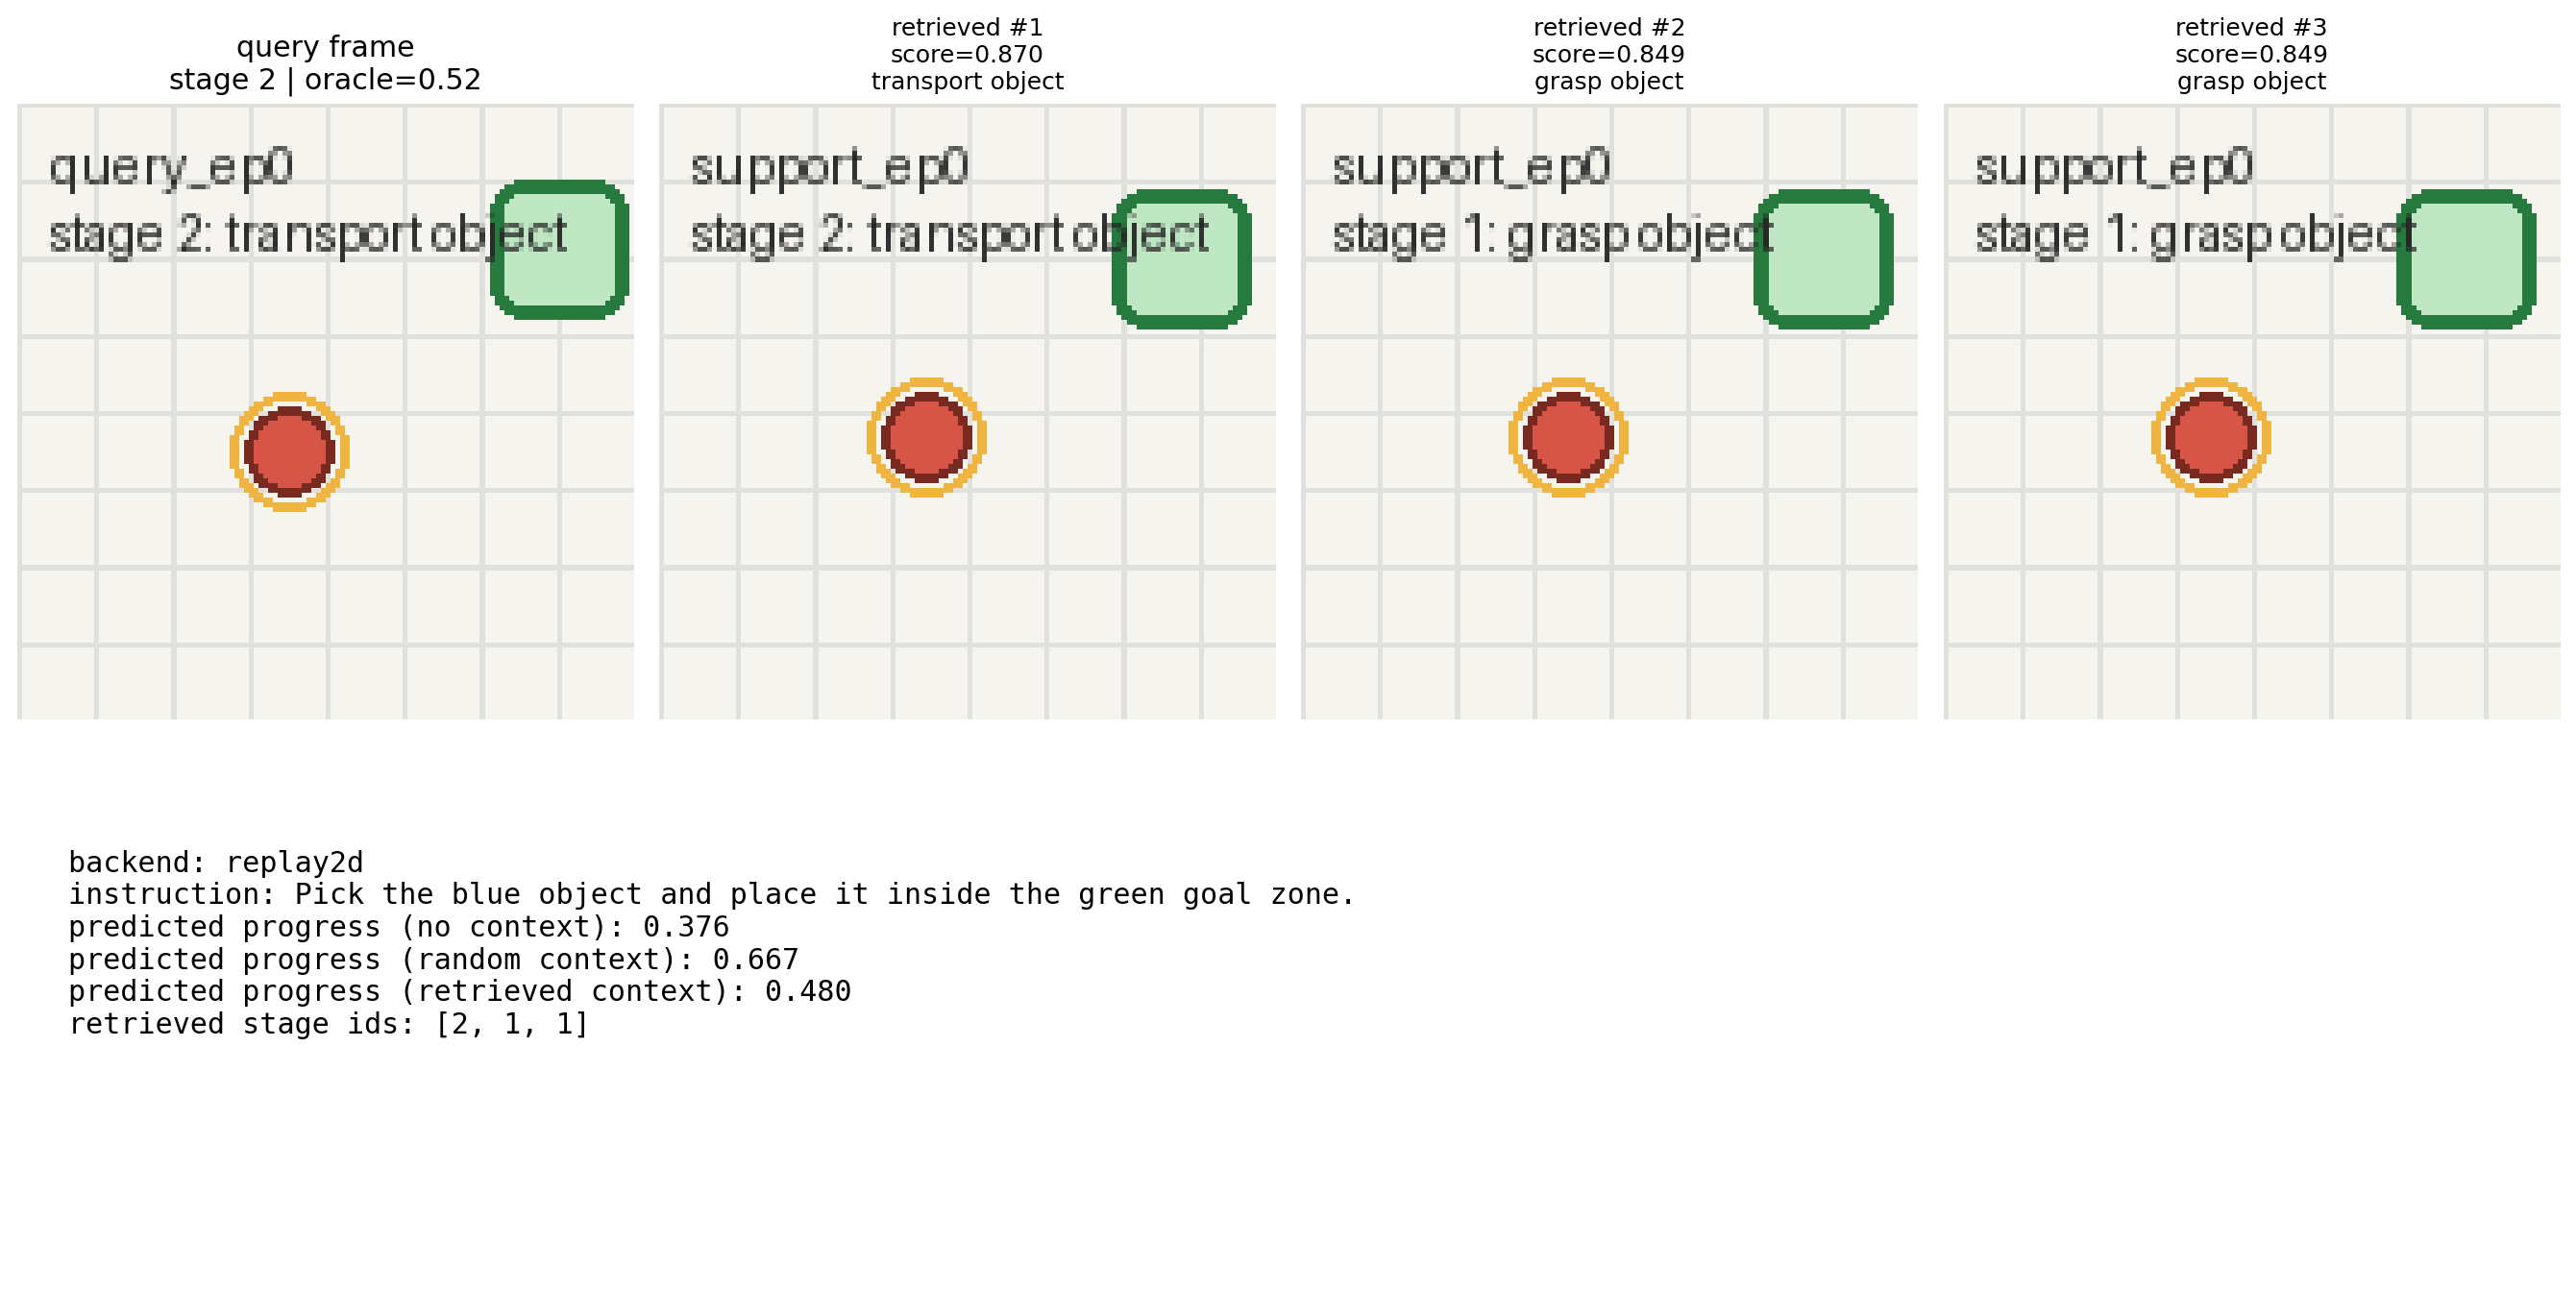
\includegraphics[width=0.76\linewidth]{../../artifacts/demo_case.png}

      \vspace{0.2em}
      {\tiny Demo snapshot with query, retrieved frames, and predicted progress}
    \end{center}
  \end{column}
\end{columns}
\end{frame}

\begin{frame}[t]{This Week's Progress: Metrics}
\small
\begin{block}{Current evidence}
  \begin{itemize}
    \item \texttt{replay2d}: \(48\) support, \(24\) query, retrieved-context MAE \(= 0.0797\), corr \(= 0.9735\)
    \item \texttt{LIBERO}: \(16\) support, \(8\) query, retrieved-context MAE \(= 0.0973\), corr \(= 0.9475\)
  \end{itemize}
\end{block}

\begin{block}{Interpretation}
  \begin{itemize}
    \item Retrieved context beats both no-context and random-context baselines.
    \item The retrieval-to-progress path already works before full reward-head training.
  \end{itemize}
\end{block}

\begin{block}{Immediate next step}
  Replace the proxy with a retrieval-conditioned reward head, then connect it to offline RL with \texttt{IQL}.
\end{block}
\end{frame}

\begin{frame}[t]{This Week's Progress: Progress Plot}
\small
\begin{columns}[T,totalwidth=\textwidth]
  \begin{column}{0.58\textwidth}
    \begin{center}
      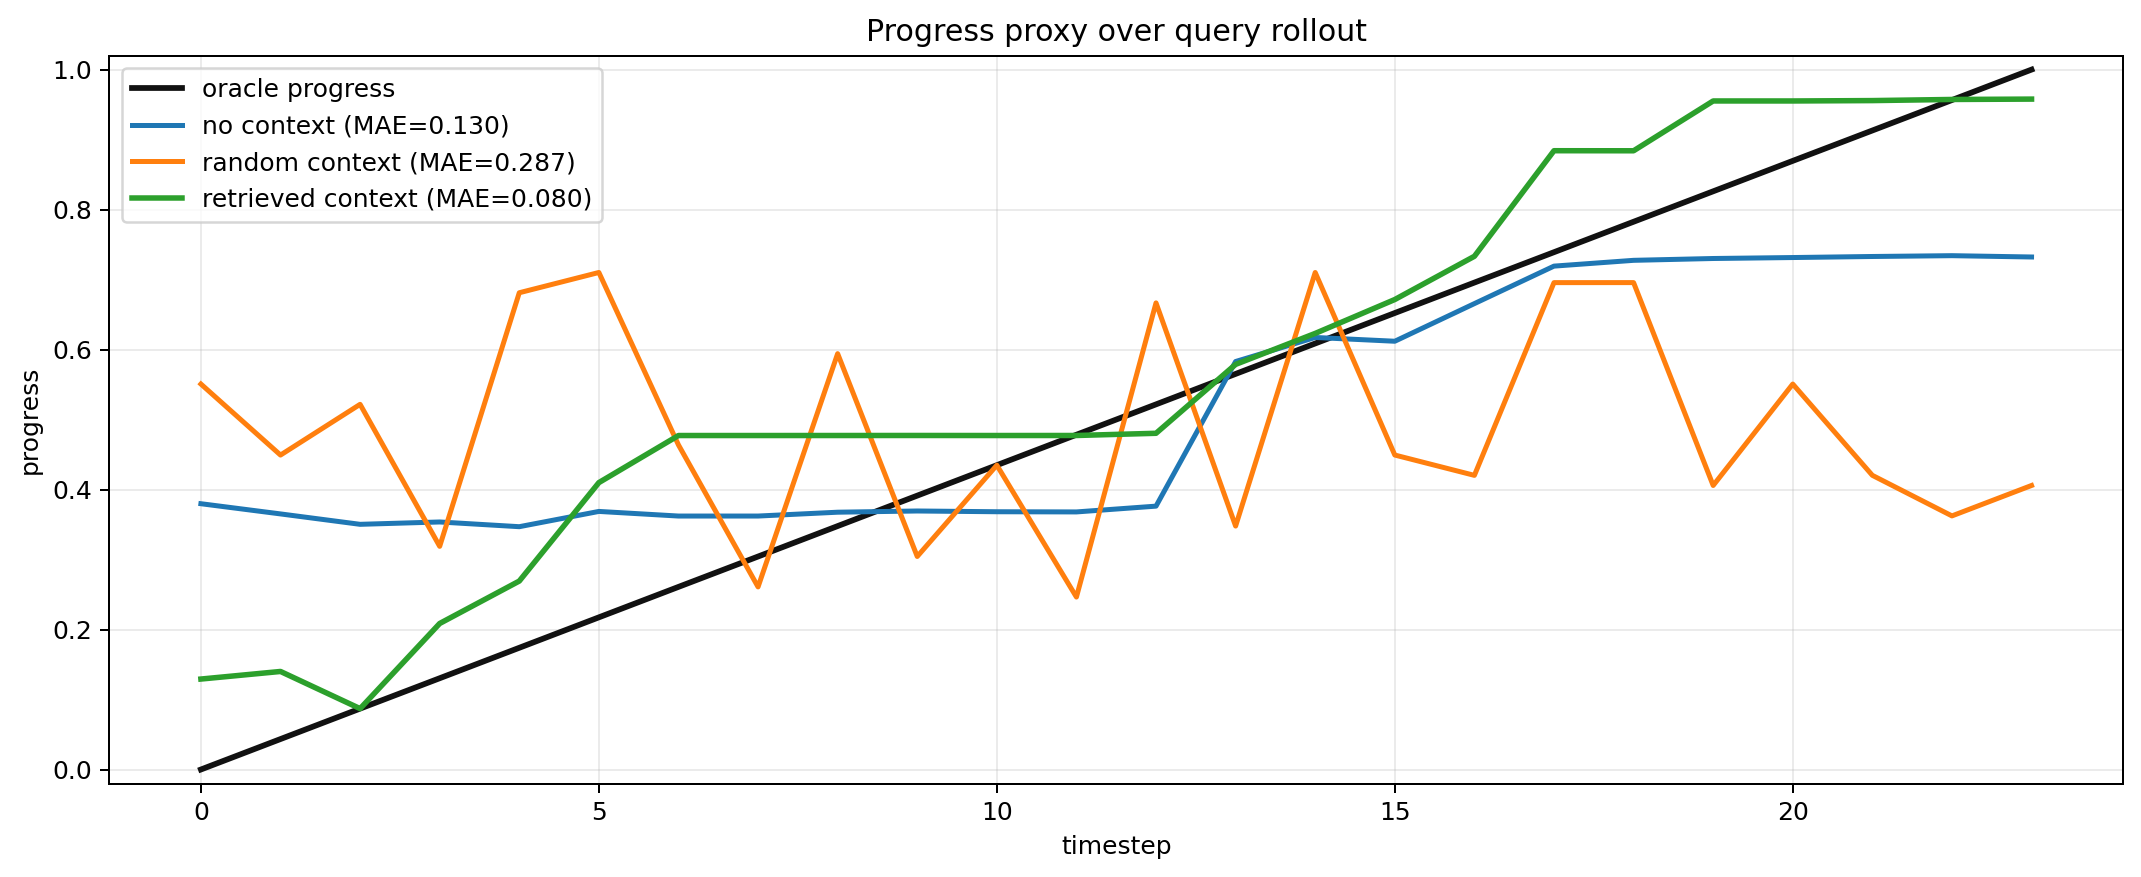
\includegraphics[width=0.96\linewidth]{../../artifacts/progress_plot.png}
    \end{center}
  \end{column}
  \begin{column}{0.38\textwidth}
    \begin{block}{How to read it}
      \begin{itemize}
        \item Oracle progress increases smoothly over time.
        \item Retrieved context tracks the oracle more closely than no context and random context.
      \end{itemize}
    \end{block}

    \begin{block}{Main takeaway}
      The prototype already shows that retrieval provides useful progress evidence before full reward-head training.
    \end{block}
  \end{column}
\end{columns}
\end{frame}

\section{Closing}
\begin{frame}[t]{Takeaway}
\small
\begin{block}{Main message}
The proposal is not claiming a vague ``robotic RAG'' system. The target is narrower and testable:
\textbf{use retrieval to improve reward quality for long-horizon manipulation in simulation, validate reward quality first, and only then move to policy learning with IQL.}
\end{block}

\begin{block}{Status today}
The project already has a working prototype that demonstrates the retrieval $\rightarrow$ progress estimation path.
This reduces risk for the next phase, which is full reward-head training and downstream offline RL.
\end{block}
\end{frame}

\begin{frame}[allowframebreaks]{References}
\tiny
\bibliographystyle{plainnat}
\bibliography{../../pdf/references}
\end{frame}

\end{document}
